\subsection{PIR Motion Sensor}\label{sub:pir}

The sensor used to detect movement is a passive infrared sensor (PIR). The model
number is \enquote{SEN32357P} and is manufactured by SEEED Studio. A data sheet
can be found in:
\cite{datasheet_pir1}. The
sensor is implemented using the \enquote{BISS0001} integrated circuit. A data sheet for this can
be found in \cite{datasheet_pir2}.

According to the technical specifications, the sensor can measure movements from 0.1 m to 6 m away. The distance can be configured by rotating a potentiometer on the sensor. Clockwise means decreasing the distance. This is essentially the sensitivity of the sensor. A smaller distance means lower sensitivity. The detecting angle is 120 degree.

The sensor also has a potentiometer for configuring the time delay. The time
delay is the time the sensor reports movement after it is detected. So
if a movement is detected, the sensor with time delay set to 10 seconds will report that motion is detected for 10 seconds after the movement.
The time delay on this specific sensor can be adjusted from 1 second to 25 seconds. A switch, on the sensor, controls whether the sensor is retriggerable (H position) or unretriggerable (L position). In a retriggerable position, the delay time is extended every time movement is detected. In the unretriggerable mode, the delay time remaining is not reset when motion is detected.

The sensor has 4 pins, GND, VCC, NC and SIG. The sensor signals motion detected on its SIG pin. LOW on this pin means no motion and HIGH means motion.

An example of a setup can be seen in \cref{fig:arduino_pir_wiring}.

\begin{figure}[htbp]
  \centering
  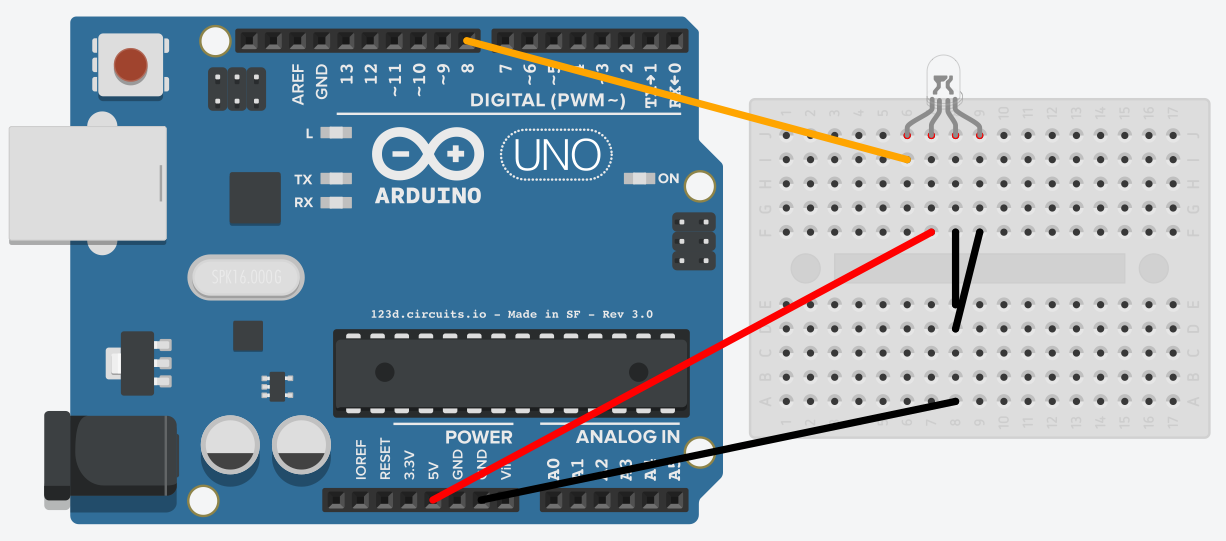
\includegraphics[width=\textwidth]{arduino-pir-wiring.png}
  \caption{The figure depicts wiring for a PIR motion sensor. A LED is shown in
    the figure, for a lack of a PIR component in the software generating the
    wiring schematics.}
  \label{fig:arduino_pir_wiring}
\end{figure}

\subsubsection{Sampling Input Data}

To reduce noise on the signal of the sensor, a simple statistical algorithm is
performed on the input data. The purpose of the algorithm is to increase reliability of the input data. Since the data can include false detection of objects that are not present, the algorithm is there to reduce  faulty data.  Essentially the data is reduced to two tiers
of data. First, the input data is accumulated into a tier1 low and a tier1 high
counter. When $n_{tier1}$ number of samples have been collected, a tier2 sampling round begins. If tier1
had more high counts than low counts, tier2 high is incremented and the opposite if
tier1 had the most lows. When the sample count of tier2 has reached a number
$n_{tier2}$, the calculated signal can be reported. If tier2 had the most highs,
report high and vice versa for tier2 lows.